% !TEX encoding = UTF-8
% !TEX TS-program = pdflatex
% !TEX root = ../tesi.tex

%**************************************************************
\chapter{Lo stage}
\label{cap:descrizione-stage}
%**************************************************************

\section{Pianificazione}
Prima dell'inizio del progetto, ho redatto assieme al tutor aziendale un piano di lavoro. All'interno di questo ho riportato gli obiettivi individuati, la pianificazione del lavoro sotto forma di processi, suddivisi a loro volta in attività. Ad ognuna di queste sono state assegnate delle ore di lavoro, la cui somma sarà il totale delle ore a disposizione per lo stage.

\bigskip

%\input{capitoli/tabella_ore} % tolta tabella in quanto sotto ho omesso la voce "Progettazione e sviluppo software CRM"

%\medskip

%DIAGRAMMA DI GANTT???

%\medskip

Le attività individuate sono:
\begin{itemize}
\item \textbf{Formazione sulle tecnologie utilizzate}: la fase iniziale dello stage consiste nella formazione sulle tecnologie usate, oggetto dei vincoli posti dall'azienda. Questa è stata una fase molto importante per poter lavorare correttamente ed in sincronia con il resto del team;

\item \textbf{Definizione del sistema hardware/software e relativa documentazione}
\begin{itemize}
	\item \textbf{Analisi del problema e del dominio applicativo}: la prima attività da svolgere è stata quella di analizzare il problema e il contesto in cui il prodotto dovrà operare. Questa attività include anche lo studio del sistema esistente in modo da comprenderne in modo esaustivo il funzionamento. Come prodotto in uscita ho ottenuto tutti i requisiti relativi alla parte hardware del progetto;
	\item \textbf{Adattamento e revisione della piattaforma esistente}: una volta compreso il funzionamento del sistema esistente e formalizzato i requisiti ottenuti dall'attività precedente, ho progettato la modifica da apportare per poter lavorare con il nuovo modulo ed in seguito ho riportato il tutto su codice;
	\item \textbf{Test piattaforma hardware}: ho pianificato ed eseguito alcuni test d'unità che andassero a verificare la correttezza sulle nuove parti di codice;
	\item \textbf{Stesura documentazione}: per poter garantire un'adeguata manutenzione al prodotto, ho redatto in questa attività tutta la documentazione relativa alle nuove modifiche;
\end{itemize}

\item \textbf{Modellazione e Stampa 3D}
\begin{itemize}
	\item \textbf{Design e modellazione involucro}: ho dedicato del tempo per la creazione digitale del modello tridimensionale per l'involucro che conterrà l'elettronica del nuovo modulo aggiunto;
	\item \textbf{Slicing del modello e stampa 3D}: ho preparato il modello creato nell'attività precedente per la stampa andando ad impostare vari parametri al computer ed infine ho provveduto alla stampa vera e propria;
\end{itemize}

\item \textbf{Sviluppo piattaforma online}
\begin{itemize}
	\item \textbf{Pianificazione e analisi dei requisiti}: ho pianificato e analizzato i requisiti per lo sviluppo della piattaforma online. Questo strumento serve al cliente finale per monitorare i vari accessi al varco controllato da FabKey e per gestire gli accessi autorizzati;
	\item \textbf{Sviluppo della piattaforma con iniziale attenzione al lato server}: a seguito della pianificazione e raccolta dei requisiti, ho proseguito con lo sviluppo della piattaforma, con priorità al lato server;
\end{itemize}

\item \textbf{Cura dell'interfaccia grafica}: ho prestato attenzione alla cura dell'interfaccia grafica relativa alla piattaforma creata nelle attività precedenti. Durante questa attività ho curato anche la parte front-end dell'applicazione online;
\item \textbf{Test e verifica presenza bug}: al termine della fase di sviluppo ho eseguito dei test sul sistema completo;
\item \textbf{Redazione dei manuali d’uso}: in questa attività ho redatto tutti i manuali d'uso sia per l'utente (uso e installazione del sistema), sia per uso interno (assemblaggio e configurazione del sistema);

\item \textbf{Collaudo Finale}
\begin{itemize}
	\item \textbf{Collaudo}: collaudo finale prima della presentazione ufficiale;
\end{itemize}
\end{itemize}

\medskip

Ho riportato gli obiettivi individuati sul piano di lavoro, categorizzandoli secondo tre tipologie come spiegato nella sezione 2.2


%**************************************************************
\section{Studio iniziale}
\subsection{Documentazione individuale}
Gli obiettivi e i vincoli fissati comprendevano alcune tecnologie e strumenti che ancora non facevano parte del mio bagaglio formativo, pertanto lo stage ha avuto inizio con una fase di studio individuale.
Supportato dal tutor aziendale e dai colleghi, ho iniziato lo studio degli strumenti che l'azienda usa regolarmente durante lo sviluppo di un progetto, come GitLab, la piattaforma online per repository Git. In precedenza, durante alcuni progetti universitari, tra i quali quello di Ingegneria del Software, ho utilizzato il software di versionamento Git tramite la piattaforma di GitHub, simile per molti aspetti a GitLab. Per questo l'apprendimento non è stato difficile.

\medskip

Ha richiesto più tempo lo studio del software di modellazione 3D Rhinoceros. Non essendomi mai approcciato al disegno e modellazione tridimensionale, apprendere le basi è stata un'operazione più lunga del previsto, ma, una volta compreso il principio alla base, la creazione di modelli semplici è un processo abbastanza intuitivo.

Ho avuto la possibilità di studiare il funzionamento della stampa 3D grazie alla disponibilità di una stampante a mio uso esclusivo. Ciò mi ha permesso di effettuare diversi test modificando i parametri di stampa e sperimentando diversi materiali, il tutto prima dello sviluppo del progetto.

\medskip

L'ultimo strumento oggetto di studio è stato Arduino. Ho iniziato studiando l'editor e le modalità di collegamento alla scheda. Prima di iniziare con dei test di funzionamento, ho preferito utilizzare il software Fritzing\footcite{http://fritzing.org/} per disegnare gli schemi di collegamento dei componenti elettronici alla scheda; questo strumento si è reso utile anche durante la redazione dei manuali ad uso interno per la guida all'assemblaggio.

\begin{figure}[H]
	\begin{center}
	\includegraphics[scale=0.62]{immagini/schema_arduino.png}
	\caption{Esempio di schema creato con Fritzing. Rappresenta uno dei primi test effettuati con scheda Arduino.}
	\end{center}
\end{figure}

\medskip

%Il progetto verrà spiegato in questa sezione, senza però scendere in dettagli, evitando quindi riproducibilità.
Lo sviluppo del progetto è partito da uno studio preliminare sul sistema già esistente composto da una centralina di controllo ed un lettore di schede NFC.
Scendendo nei dettagli, la fase di studio è iniziata dalla centralina, composta da una scheda Arduino. Per poterne apprendere il funzionamento, il tutor aziendale mi ha fornito una scheda di test sulla quale eseguire del codice di esempio con dei semplici circuiti elettronici. L'apprendimento si è rivelato piuttosto rapido anche grazie alla vasta disponibilità di materiale online e ad una consolidata community.

Una volta appreso il funzionamento generale di Arduino, ho iniziato lo studio sul codice che governa il comportamento della centralina di controllo, caratterizzato principalmente da 3 fasi:

\begin{itemize}
\item \textbf{Configurazione iniziale}: il sistema esegue una configurazione iniziale in modo da integrarsi perfettamente nella rete alla quale è collegato;
\item \textbf{Listener}: una porzione di codice che rimane in continuo ascolto per catturare gli eventi derivanti dai moduli collegati;
\item \textbf{Crittografia e HTTP request}: una funzione che si occupa della cifratura dei codici letti e del loro invio tramite richieste HTTP ad un server.
\end{itemize}

Terminata questa prima fase di studio, è susseguita quella di analisi.

\section{Analisi dei requisiti}
\subsection{Identificazione}
Per poter identificare correttamente tutti i requisiti, a seguito di vari colloqui con il tutor aziendale e il cliente, ho definito i vari casi d'uso, disegnandone in seguito i rispettivi diagrammi UML. Ogni riunione è stata riportata su di un verbale e da quest'ultimo ho in seguito ricavato i vari requisiti. Ho anche analizzato approfonditamente i casi d'uso in modo da poter identificare ulteriori requisiti. Una volta individuati tutti i requisiti sono stati riportati in un documento soggetto a versionamento.

\subsection{Strumenti a supporto}
\subsubsection{Casi d'uso}
I casi d'uso e i relativi diagrammi UML sono stati un ottimo strumento di supporto durante la fase di analisi: mi hanno permesso di individuare alcuni requisiti non emersi durante le riunioni con tutor e stakeholders.

\begin{figure}[H]
	\begin{center}
	\includegraphics[scale=0.4]{immagini/usecase/scenario_principale.png}
	\caption{Estratto dello schema UML rappresentante i casi d'uso dello scenario principale. Schema riferito all'uso di FabKey e non alla piattaforma online.}
	\end{center}
\end{figure}

Essendo il progetto composto da due sistemi, FabKey e piattaforma online, i casi d'uso sono stati categorizzati da una notazione univoca, che facilita l'identificazione del caso d'uso nel contesto:

\begin{center}
\textbf{UC\textunderscore [Contesto].[IDUnivoco]}
\end{center}

\begin{itemize}
\item \textbf{Contesto}:
\begin{itemize}
\item \textbf{FK}: FabKey;
\item \textbf{PO}: Piattaforma online di gestione.
\end{itemize}

\item \textbf{IDUnivoco}: Un codice numerico progressivo che identifica in maniera univoca il caso d'uso a cui si riferisce. Questo codice può essere gerarchico in modo da identificare casi d'uso innestati.
\end{itemize}

\begin{figure}[H]
	\begin{center}
	\includegraphics[scale=0.4]{immagini/usecase/UC_FK_4.png}
	\caption{Dettaglio del caso d'uso UC\textunderscore FK.4. Si può notare l'uso della notazione sopra descritta.}
	\end{center}
\end{figure}

Ogni caso d'uso ha una specifica provenienza, ovvero alcune determinate fonti che lo hanno generato.
Queste sono:
\begin{itemize}
\item \textbf{Verbali}: ottenuti trascrivendo quanto emerso durante i colloqui con i portatori di interesse;
\item \textbf{Le specifiche del sistema}: descrivono quali sono le caratteristiche che il sistema deve avere;
\item \textbf{Conoscenza del dominio}: la conoscenza del contesto d'utilizzo e la consultazione di materiale ad esso inerente.
\end{itemize}

Ho utilizzato queste fonti anche per l'identificazione dei requisiti.

\subsection{Formalizzazione dei requisiti}
Dopo aver individuato tutti i requisiti necessari allo sviluppo del progetto, ho creato una codifica che li potesse identificare in maniera univoca e allo stesso tempo catalogare per tipo e priorità.
La codifica utilizzata è la seguente:

\begin{center}
\textbf{R[Componente]\textunderscore [Tipologia]\textunderscore [Priorità][Numero Identificativo]}
\end{center}

\textbf{Componente}
\begin{itemize}
\item \textbf{FK}: requisito inerente allo sviluppo della parte elettronica di FabKey;
\item \textbf{PO}: requisito relativo allo sviluppo del portale online per la gestione degli accessi.
\end{itemize}

\textbf{Tipologia}
\begin{itemize}
\item \textbf{F}: un requisito di tipo funzionale, cioè che aggiunge funzionalità al sistema;
\item \textbf{Q}: requisito di qualità, ovvero che, se soddisfatto, aumenta la qualità generale del prodotto;
\item \textbf{P}: requisito prestazionale, mirato a migliorare il prodotto in termini di prestazioni.
\end{itemize}

\textbf{Priorità}
\begin{itemize}
\item \textbf{Ob}: requisiti obbligatori, il cui sviluppo è condizione necessaria per ottenere il risultato finale;
\item \textbf{De}: requisiti desiderabili, ovvero soddisfarli significa apportare importanti miglioramenti al prodotto anche se non strettamente vincolanti al suo funzionamento;
\item \textbf{Op}: requisiti opzionali, che apportano valore aggiunto al sistema, ma il cui sviluppo è trascurabile.
\end{itemize}

\textbf{Numero Identificativo}

\medskip

Un codice numerico progressivo che identifica in maniera univoca il requisito a cui si riferisce. Questo codice può essere gerarchico.

\bigskip

Riporto di seguito alcuni dei requisiti individuati:

\medskip

\textbf{Hardware FabKey}
\renewcommand{\arraystretch}{2.0}
\begin{longtable}{|l|p{2.5cm}|p{8cm}|}
\hline
\textbf{Codice} & \textbf{Tipo} & \textbf{Descrizione} \\ 
\hline
\textbf{RFK\_F\_Ob1} & Funzionale \linebreak Obbligatorio & Il sistema deve permettere la lettura di un codice a barre \\ 
\hline
\textbf{RFK\_F\_Ob2} & Funzionale \linebreak Obbligatorio & Il sistema deve attivare il lettore quando rileva un utente nelle vicinanze \\
\hline
\textbf{RFK\_Q\_Ob1} & Qualità \linebreak Obbligatorio & Il modulo di lettura deve essere contenuto in un involucro stampato in 3D \\
\hline
\textbf{RFK\_Q\_Op1} & Qualità \linebreak Opzionale & L'involucro esterno deve essere modulare ed espandibile per versioni successive \\
\hline
\caption{Alcuni requisiti individuati per lo sviluppo della parte hardware di FabKey.}
\end{longtable}


\medskip

\textbf{Portale online}
\renewcommand{\arraystretch}{2.0}
\begin{longtable}{|l|p{2.5cm}|p{8cm}|}
\hline
\textbf{Codice} & \textbf{Tipo} & \textbf{Descrizione} \\ 
\hline
\textbf{RPO\_F\_Ob1} & Funzionale \linebreak Obbligatorio & L'applicazione deve permettere di visualizzare l'elenco degli utenti autorizzati \\ 
\hline
\textbf{RPO\_F\_Ob2} & Funzionale \linebreak Obbligatorio & L'applicazione deve permettere di gestire le autorizzazioni \\
\hline
\textbf{RPO\_F\_Ob2.1} & Funzionale \linebreak Obbligatorio & L'applicazione deve permettere di eliminare un'autorizzazione \\
\hline
\textbf{RPO\_F\_De1} & Funzionale \linebreak Desiderabile & L'applicazione deve presentare un'interfaccia grafica completamente scalabile \\
\hline
\caption{Alcuni requisiti individuati per lo sviluppo del gestionale online di FabKey.}
\end{longtable}


Dopo aver individuato e codificato tutti i requisiti, ho composto una tabella in cui ho riportato il tracciamento tra i requisiti e i casi d'uso, in modo da identificare in quale caso d'uso viene soddisfatto un determinato requisito.

\section{Progettazione}
\subsection{L'approccio iniziale}
Ho gestito la progettazione del prodotto in modo separato rispetto alle due componenti principali che ne fanno parte: l'hardware di FabKey (composto da centralina e lettore) e l'applicazione online per la gestione delle autorizzazioni. Per comodità chiamerò queste due componenti \textbf{HWFabKey} e \textbf{Gestionale accessi} rispettivamente.

\medskip

La fase di progettazione è stata molto importante, in quanto la sua corretta realizzazione mi avrebbe permesso una fase di codifica rapida minimizzando i rischi di errore.

\bigskip

\subsection{Progettazione di HWFabKey}

Le componenti alle quali dovevo prestare particolare attenzione durante la fase di progettazione erano quattro:
\begin{itemize}
\item \textbf{Gestione delle componenti elettroniche che compongono il lettore di codice a barre}: durante la progettazione ho ideato lo schema per i collegamenti del lettore di codici a barre (composto da diverse componenti elettroniche), prestando attenzione a non creare interferenze con altre componenti già collegate nella versione esistente, come ad esempio il circuito apri porta;
\item \textbf{Sicurezza nella trasmissione dei dati}: i dati trasmessi verso il server andavano crittografati per evitare di incorrere in alcuni problemi di sicurezza;
\item \textbf{Protocollo di comunicazione con il server}: dovevo scegliere in questa fase il modo in cui la centralina avrebbe comunicato con il server, analizzando pro e contro delle varie alternative.
\item \textbf{Creazione e stampa 3D dell'involucro}: dopo aver abbozzato su carta alcune ipotesi e averne discusso le caratteristiche con il tutor, ho disegnato e stampato in 3D l'involucro;
\end{itemize}

\begin{figure}[H]
	\begin{center}
	\includegraphics[scale=0.4]{immagini/schema_labkey.jpg}
	\caption{Schema di funzionamento di FabKey.}
	\small{\textbf{Fonte:} \url{https://www.labkey.it}}
	\end{center}
\end{figure}

\subsubsection{Gestione dell'elettronica}
L'utilizzo del nuovo modulo per la lettura di codici a barre ha comportato la gestione di 4 nuove componenti elettroniche, le quali andavano collegate ad Arduino senza interferire con le componenti base del sistema.
Ho risolto tutto questo disegnando lo schema completo ed aiutandomi con un simulatore.

\begin{figure}[H]
	\begin{center}
	\includegraphics[scale=0.065]{immagini/lettore_barcode.jpg}
	\caption{Una delle componenti elettroniche che compongono il lettore di codici a barre. Si tratta del vero e proprio lettore ottico.}
	\end{center}
\end{figure}

\subsubsection{Sicurezza nella trasmissione dati}
Il maggior problema che ho riscontrato nella gestione della trasmissione dei dati è stato quello riguardante la sicurezza. A primo impatto ho pensato all'uso di una codifica con funzioni crittografiche hash, come ad esempio MD5 o SHA-1, ma non avevo preso in considerazione un aspetto molto importante: la memoria disponibile. 

\begin{figure}[H]
	\begin{center}
	\includegraphics[scale=0.4]{immagini/hash.png}
	\caption{Esempio di funzione hash. Risultato dei primi quattro byte della funzione hash SHA-1.}
	\small{\textbf{Fonte:} \url{https://it.wikipedia.org/wiki/Hash}}
	\end{center}
\end{figure}

Nell'hardware a disposizione le risorse erano estremamente limitate: avevo tralasciato questo aspetto dal momento che ho sempre lavorato con dispositivi la cui potenza di calcolo era trascurabile per questo tipo di operazioni. Nel caso specifico, 2 KB di memoria SRAM non erano sufficienti per la gestione dell'intero programma di controllo e contemporaneamente memorizzare una variabile di 40 byte o più, contenente la stringa con codifica hash. Per cui, collaborando con un collega, abbiamo ideato un algoritmo di crittografia semplificato, basato sul principio della funzione hash, ma in grado di produrre un output nettamente ridotto.


\subsubsection{Protocollo di comunicazione}
Uno dei requisiti prevedeva lo scambio di informazioni tra la centralina di controllo, connessa in rete tramite cavo LAN, e il server centrale, contenente il database con gli accessi autorizzati.
Il compito del team era di soddisfare questo requisito in modo che la comunicazione fosse il più rapida possibile.
La soluzione adottata consiste in una semplice chiamata HTTP verso il server: viene creato un \textit{URL} composto dall'indirizzo del server e il codice di accesso richiesto, codificato tramite l'algoritmo sopra descritto; il server, ricevuta la richiesta, ricava dall'\textit{URL} il codice crittografato e lo confronta con i dati presenti nel database, rispondendo con un segnale positivo o negativo.

\begin{figure}[H]
	\begin{center}
	\includegraphics[scale=0.37]{immagini/comunicazione_http.png}
	\caption{Schema di comunicazione Centralina/Server.}
	\end{center}
\end{figure}

\subsubsection{Progettazione dell'involucro e stampa 3D}
L'idea era di realizzare un involucro in grado di contenere tutte le componenti elettroniche del lettore e che fosse allo stesso tempo il più compatto possibile.
Per prima cosa ho abbozzato dei disegni con alcune ipotesi sulle forme generali e, una volta approvato dal tutor, ho iniziato la creazione del modello tridimensionale.

\begin{figure}[H]
	\begin{center}
	\includegraphics[scale=0.37]{immagini/render.png}
	\caption{La prima versione dell'involucro per il lettore di codici a barre.}
	\end{center}
\end{figure}

Una volta ottenuto il modello finito, ho configurato il processo di stampa grazie al software open source Cura di Ultimaker. Grazie a questa applicazione è possibile, dopo aver impostato i diversi parametri, simulare la stampa, in modo da verificare eventuali errori di configurazione o sul modello.

\begin{figure}[H]
	\begin{center}
	\includegraphics[scale=0.37]{immagini/simulatore_stampa.png}
	\caption{Un componente dell'involucro durante la simulazione con il software Cura.}
	\end{center}
\end{figure}

%Progettazione online app
% Si potrebbe inserire un grafico che rappresenti il database MySql
%ragioni della scelta del db relazionale

\subsection{Progettazione del gestionale accessi}
L'applicazione web per la gestione delle autorizzazioni è composta da un lato front-end e da un lato back-end. La prima parte è formata dall'interfaccia grafica e dalle componenti lato client, mentre la seconda contiene il database e le funzioni per l'elaborazione della risposta alle chiamate http da parte della centralina.

\subsubsection{Front-end - Interfaccia grafica}
Facendo riferimento ai casi d'uso, ho iniziato a progettare l'interfaccia grafica della WebApp, definendo le varie sezioni di cui sarà composta.
Ho previsto un menù di navigazione laterale contenente i collegamenti a tutte le pagine presenti.

\begin{figure}[H]
	\begin{center}
	\includegraphics[scale=0.32]{immagini/dashboard_crm.png}
	\caption{Schermata principale del gestionale.}
	\end{center}
\end{figure}

Le sezioni presenti sono:
\begin{itemize}
\item \textbf{Schermata di login}: per poter accedere all'applicazione è necessario collegarsi al sistema con le proprie credenziali ed è possibile effettuarlo in questa schermata;
\item \textbf{Dashboard}: rappresenta la pagina iniziale dopo il login; fornisce all'utente alcune informazioni generali sul sistema, ad esempio il numero di utenti attivi, i varchi, gli accessi effettuati in giornata e una statistica sugli accessi;
\item \textbf{Utenti}: è la pagina che permette la gestione degli utenti con operazioni di inserimento, modifica, eliminazione e assegnazione di una chiave;
\item \textbf{Strutture}: l'applicazione permette tramite questa pagina la gestione di strutture geograficamente dislocate permettendo di aggiungerne di nuove, eliminare le presenti o modificarle;
\item \textbf{Varchi}: i varchi rappresentano le porte di una struttura, pertanto ogni varco è associato ad una struttura;
\item \textbf{Utenti Varchi}: è la sezione che permette di assegnare un utente ad uno o più varchi; in parole povere l'utente può definire quale utente può attraversare determinate porte;
\item \textbf{Accessi}: viene proposto in questa pagina un log degli accessi effettuati con dettagli su utente, varco e orario dell'accesso.
\end{itemize}

\begin{figure}[H]
	\begin{center}
	\includegraphics[scale=0.32]{immagini/accessi_crm.png}
	\caption{Schermata del pannello di controllo degli accessi.}
	\end{center}
\end{figure}

\subsubsection{Back-end - Database}
Per la raccolta dei dati abbiamo scelto di creare un database di tipo relazionale SQL.
Ho previsto assieme al team la creazione di tabelle che andassero a rappresentare i vari elementi caratterizzanti del sistema: gli utenti, i varchi, le strutture e alcune tabelle di collegamento per le relazioni di tipo N-N.
Essendo una tecnologia a me già nota, è stata relativamente semplice la progettazione logica del database, portata a termine con il supporto di appositi schemi E-R.

\subsubsection{Back-end - Funzione di risposta}
Parte dell'applicazione è la funzione che gestisce le richieste da parte della centralina. Il principio di funzionamento di questa procedura è relativamente semplice: alla richiesta HTTP della centralina viene estrapolata la chiave crittografata e il varco dal quale è arrivata la richiesta; successivamente si confrontano queste informazioni con i record presenti nel database tramite una query SQL e viene fornita una risposta positiva o negativa. 

\section{Codifica e realizzazione}
\subsection{Tecnologie e linguaggi}
% html, css, javascript, php, mysql, c, bootstrap (o wordpress), librerie Arduino
La fase di codifica consiste nell'implementazione di tutte le componenti definite durante la fase di progettazione, applicando le tecnologie selezionate.

Per prima cosa ho iniziato la codifica della centralina Arduino, le tecnologie coinvolte sono state:

\begin{itemize}
\item \textbf{Arduino IDE e linguaggio C}: per la programmazione del microcontrollore ATMega presente nella scheda Arduino, ho usato l'IDE fornito da Arduino stesso e il linguaggio di programmazione richiesto è il C. Nonostante fossi già ad un buon livello di conoscenza di programmazione con linguaggio C, la trascrizione in codice di quanto progettato non è stata immediata, questo a causa delle diverse librerie da utilizzare, le cui funzioni andavano studiate nel comportamento.
\item \textbf{Librerie Arduino}: ogni particolare componente elettronico disponeva di una specifica libreria per controllarne il funzionamento. Prima di iniziare la codifica finale ho dovuto studiare le funzioni specifiche di queste librerie che sarei andato ad utilizzare.
\begin{itemize}
	\item \textbf{SPI}: \textit{Serial Peripheral Interface} è un protocollo per la comunicazione seriale sincrona usata per la comunicazione tra microcontrollori. Nello specifico ho utilizzato le funzionalità di questa libreria per la comunicazione tra Arduino Uno e il lettore di codici a barre;
	\item \textbf{Ethernet}: la centralina è dotata di un modulo aggiuntivo che la equipaggia di una porta Ethernet. L'apposita libreria per l'utilizzo di questa porta è necessaria per la configurazione di rete;
	
\end{itemize}
\end{itemize}

La traduzione del progetto in codice in questo frangente non è stato per me difficoltoso: ho riscontrato, invece, maggiori problematiche durante la verifica del software, in seguito al caricamento sulla scheda Arduino. Grazie ad alcuni test, ho evidenziato che il codice si comportava saltuariamente in maniera anomala rispetto a quanto previsto, creando un flusso in output apparentemente casuale: ho scoperto in seguito che venivano creati dei caratteri casuali in uscita a causa di interferenze provocate dalla comunicazione seriale con il lettore di codici a barre. Il problema è stato risolto apportando alcune modifiche al software, in modo da ignorare questi caratteri dannosi. I test effettuati sono spiegati nella sezione\textbf{~\ref{test}}.

\medskip

La seconda parte della codifica è stata incentrata sulla creazione del gestionale e le tecnologie utilizzate sono le seguenti:

\begin{itemize}
\item \textbf{PHP e Laravel}: per la codifica della componente back-end del gestionale ho utilizzato il linguaggio PHP con il framework Laravel, caratterizzato da un pattern di tipo Model-View-Controller. Per la gestione del Controller ho sfruttato il supporto fornito da CRUDBooster, un CRUD (Create, Read, Update, Delete) generator che, tramite un sistema a ``scaffolding'', automatizza la creazione di oggetti e interfacce. Queste per me sono state tecnologie nuove e hanno richiesto un periodo di studio individuale precedente alla fase di codifica.
	\begin{itemize}
		\item \textbf{Bootstrap}: è un framework front-end per la creazione di componenti lato client, integrato nel framework Laravel. Ho utilizzato la struttura messa a disposizione da Bootstrap per la creazione delle viste.
	\end{itemize}
\end{itemize}

\subsection{Segnalazione bug e relativa risoluzione}
Non di rado accadeva durante la codifica di riscontrare alcuni bug, oppure di dover integrare alcune caratteristiche al sistema non previste nella progettazione. A questo proposito, durante la fase di progettazione, il team assieme al tutor, aveva concordato una procedura per la gestione di queste situazioni tramite la piattaforma di \textit{GitLab}. Il componente del team che riscontrava un bug o riportava la richiesta di aggiungere nuove funzionalità doveva:
\begin{itemize}
\item Creare un nuovo \textit{issue} fornendo un titolo breve ma esaustivo e una descrizione completa di tutti i dettagli allegando, se necessario, schermate o porzioni di codice. Chi avrebbe letto l'issue avrebbe dovuto essere in grado di interpretarlo senza dover approfondire con chi l'aveva creato;
\item Selezionare un assegnatario, che avrebbe avuto l'onere di risolvere il bug, con la possibilità di assegnare l'issue anche a se stessi;
\item Etichettare l'issue con una o piu \textit{labels}, per identificare il tipo di problema riportato; nel caso di un problema nella codifica andava riportata la label ``bug'', oppure per l'aggiunta di nuove funzionalità ``enhancement'';
\item Eventualmente, era possibile creare un nuovo branch nel caso di aggiunta di nuove funzionalità isolate dal branch master;
\end{itemize}

\subsection{Stampa 3D}

\medskip

Per completare il prodotto ho realizzato il primo prototipo di involucro con la stampante 3D. 

La procedura per la stampa 3D di un modello, come già sperimentato durante lo studio preliminare, consisteva di tre passaggi strettamente sequenziali:
\begin{itemize}
\item \textbf{Pre-riscaldamento e caricamento del materiale}: tramite il pannello di controllo della stampante, dovevo portare in temperatura il piano di stampa a 60 °C e l'ugello di estrusione a 200 °C. Successivamente andava caricato il filamento di materiale che avrei utilizzato per la creazione del modello: le temperature selezionate erano adatte per l'utilizzo di un materiale chiamato PLA (acido polilattico).
\end{itemize}

\begin{figure}[H]
	\begin{center}
	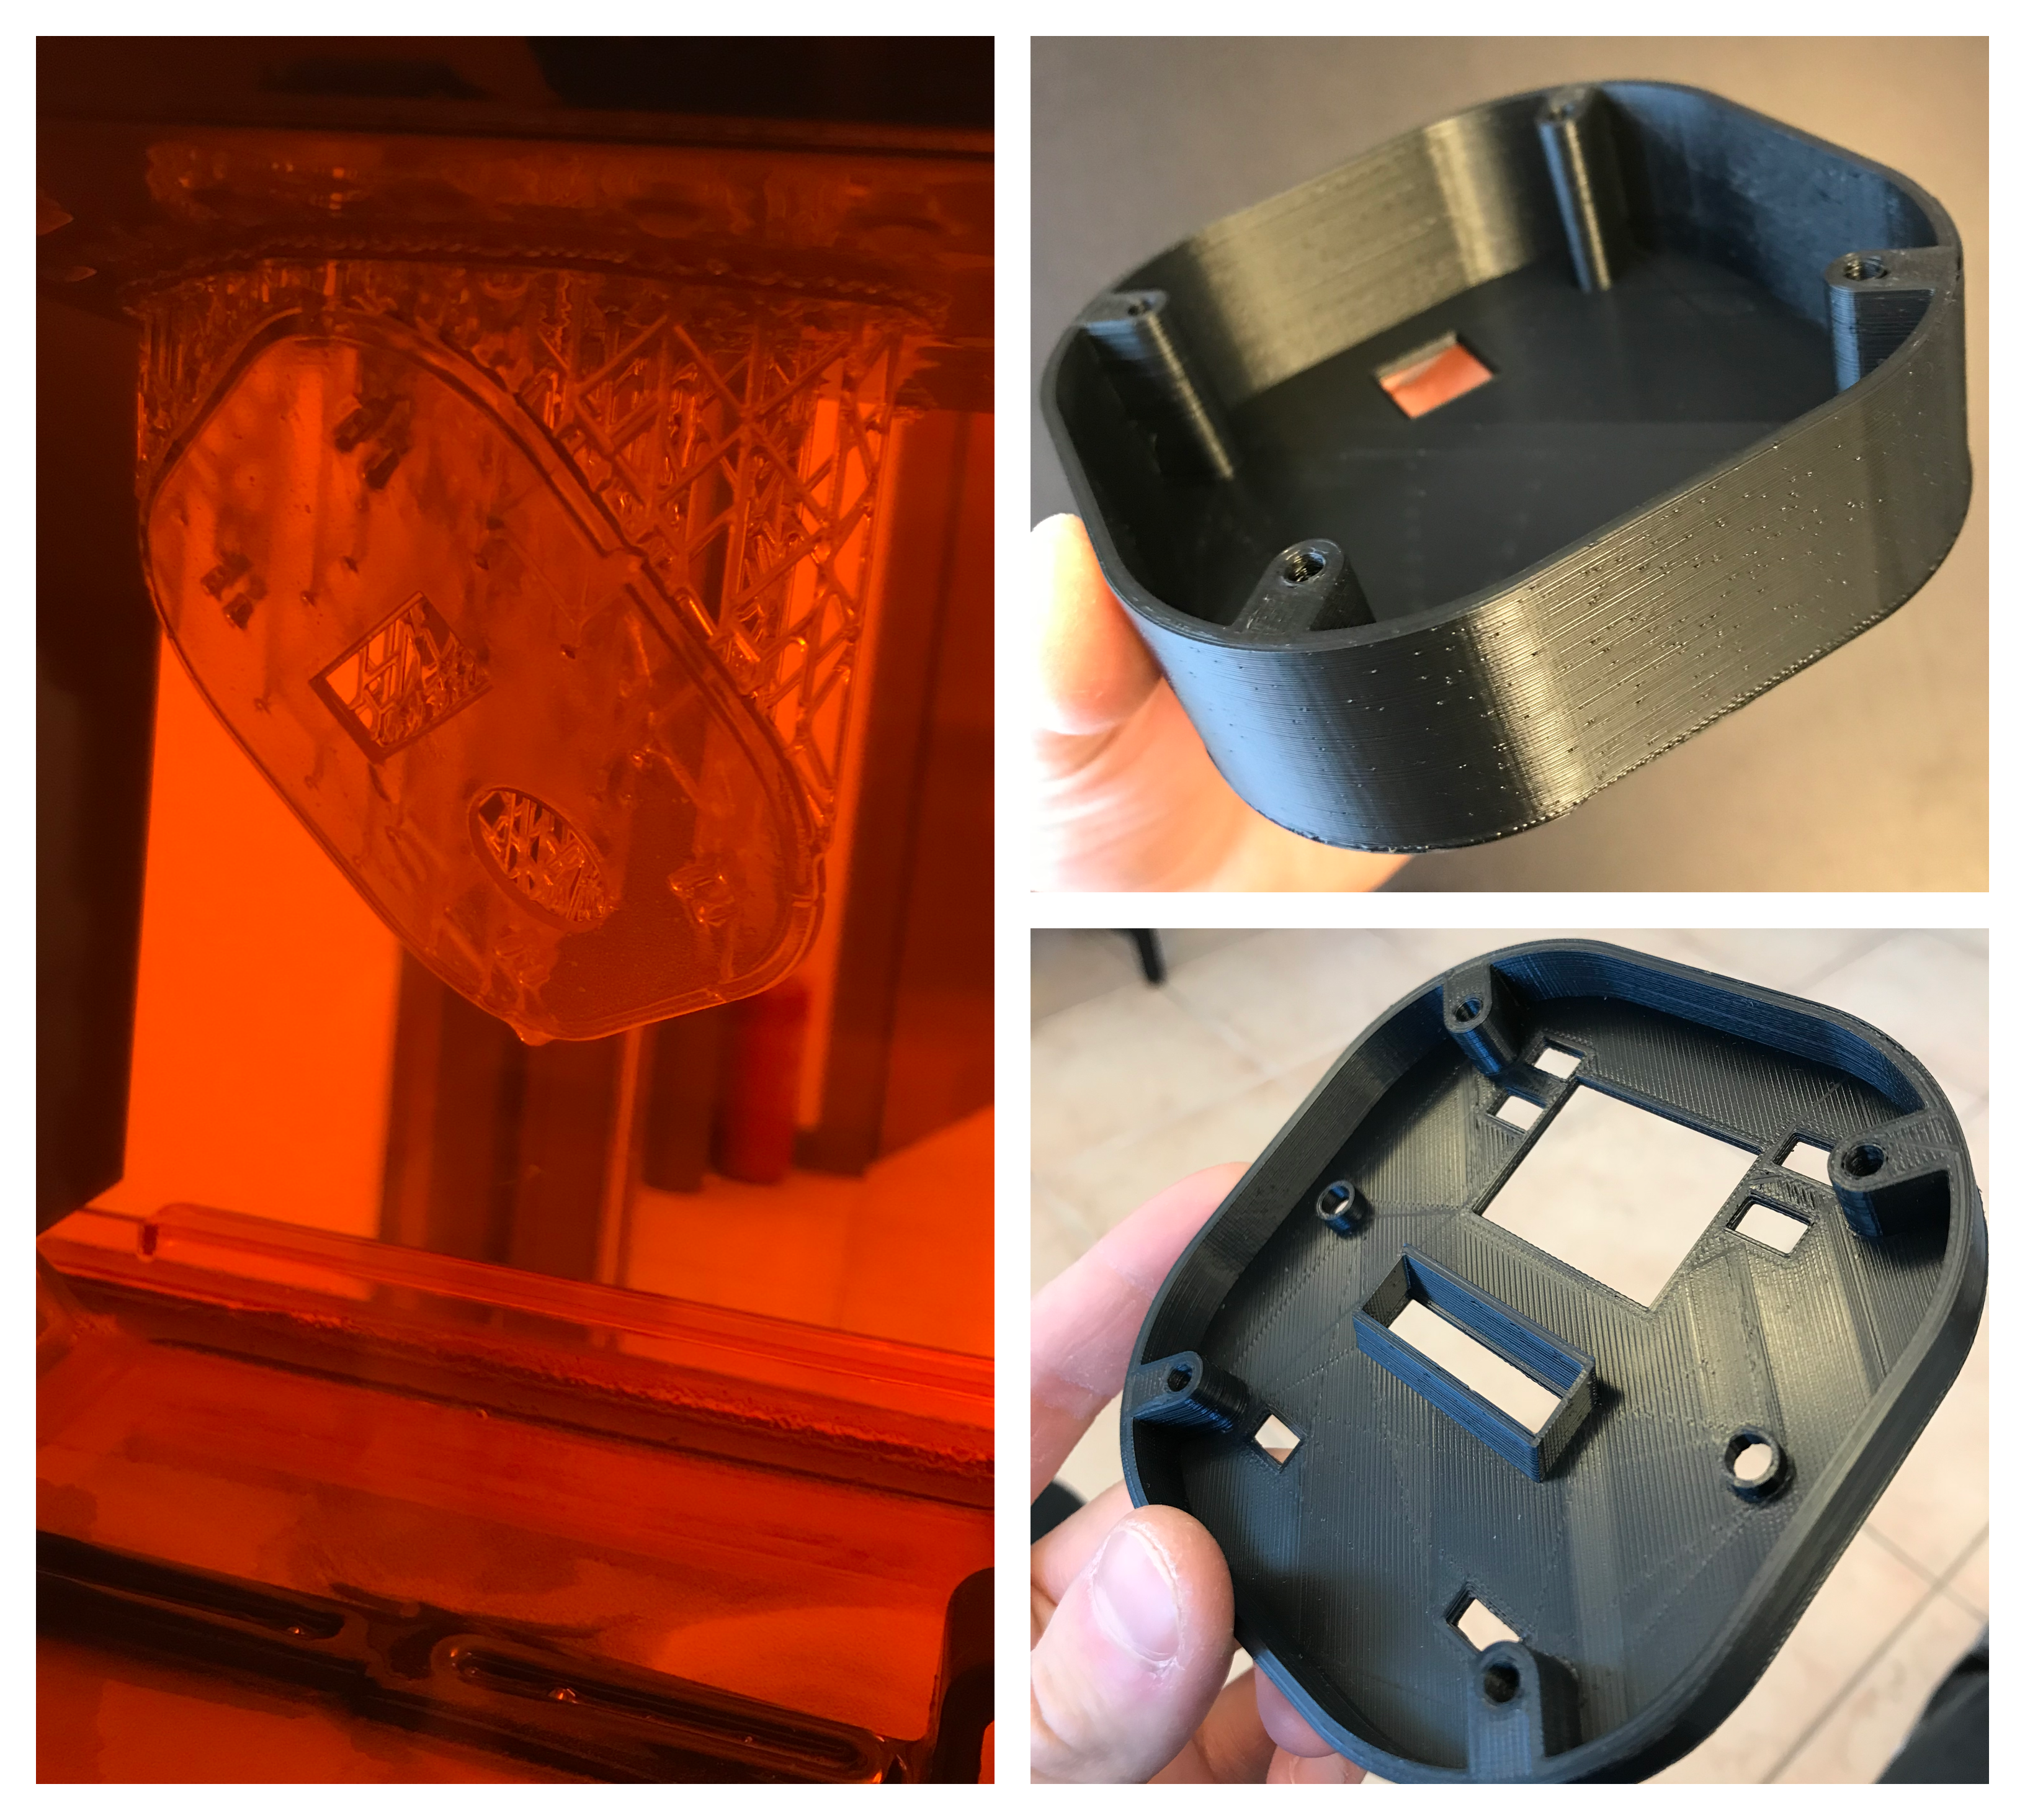
\includegraphics[scale=0.07]{immagini/stampa_3d_finale.jpg}
	\caption{I primi prototipi di involucro stampati in 3D.}
	\end{center}
\end{figure}

Con l'involucro a disposizione ho potuto procedere con l'assemblaggio finale di tutte le componenti elettroniche, terminando così la prima versione del prodotto. A codifica completata, ho concluso con la preparazione dei test di sistema e successivamente con la loro esecuzione.

\subsection{Redazione dei manuali}
I requisiti richiedevano anche la redazione dei manuali, necessari all'utente e al personale interno, per un corretto utilizzo del sistema:
\begin{itemize}
\item \textbf{Manuale d'uso utente}: questo manuale è stato scritto per guidare l'utente finale all'utilizzo sia della piattaforma online per la gestione degli utenti, che per l'utilizzo del sistema di apertura porta;
\item \textbf{Manuale di installazione}: breve guida per l'installatore dove sono riportate le istruzioni per la corretta installazione delle componenti elettriche quali centralina e lettore esterno;
\item \textbf{Manuale di configurazione}: questo è un manuale ad uso interno, il suo scopo è di guidare il tecnico durante l'assemblaggio delle componenti elettroniche e la configurazione software, operazioni previste prima della consegna al cliente;
\end{itemize}

Per la scrittura dei manuali ho utilizzato \LaTeX, un linguaggio di markup utilizzato per la stesura di testi.
Ho effettuato questa scelta per alcuni motivi in particolare:
\begin{itemize}
\item \textbf{Buona conoscenza del linguaggio}: ho spesso usato questo linguaggio per la stesura dei documenti di alcuni progetti universitari, per cui disponevo già di una buona conoscenza nel suo utilizzo;
\item \textbf{Indici e riferimenti}: facilità, flessibilità ed efficienza nella creazione degli indici e dei riferimenti incrociati; occupandosi solamente del contenuto, questo tipo di strutture vengono generate automaticamente;
\item \textbf{Gestione versionamento}: si integra perfettamente con software per il controllo della versione (Git, SVN, ...) permettendo di gestire facilmente le versioni del documento, come se fosse un software. La sua struttura permette inoltre a più utenti di lavorare contemporaneamente a diverse parti del documento.
\end{itemize}

\section{Verifica e validazione}
\subsection{Test}\label{test}
Al fine di collaudare e validare il prodotto ho previsto diversi test di unità e di sistema per verificare la correttezza di porzioni di codice e la loro integrazione nel sistema completo. I test di unità, a differenza di quelli di sistema, sono stati eseguiti anche durante la fase di codifica, in modo da segnalare ed eliminare tempestivamente la presenza di eventuali bug.
\subsubsection{Test del codice di Arduino}
Effettuare dei test di unità direttamente sulla scheda Arduino avrebbe dato vita ad un processo ripetitivo e lento composto da:
\begin{itemize}
\item Modifica del codice;
\item Compilazione e caricamento sulla scheda Arduino;
\item Osservazione del comportamento e trarre ipotesi sul suo funzionamento, positivo o negativo che sia;
\item Ripetere i passaggi.
\end{itemize}

Per questo motivo ho deciso di testare la qualità del codice scritto facendolo eseguire direttamente al computer. 
I test di unità che ho previsto avevano la seguente struttura:
\begin{enumerate}
\item Per prima cosa ho isolato la parte di codice di interesse, rendendola eseguibile come programma esterno;
\item Ho composto una previsione di output anche relazionata all'eventuale input fornito all'unità;
\item Nel caso in cui la porzione di codice effettuasse chiamate a funzioni di librerie esterne, ho creato dei mock-up che avrebbero simulato il comportamento di tali procedure, in modo da testare esclusivamente la qualità del codice scritto da me;
\item Dopo l'esecuzione del test, se l'output corrispondeva alle attese si procedeva al caricamento del test sulla scheda Arduino, altrimenti si modificava il codice in modo da correggerlo;
\item Se il comportamento del codice eseguito sulla scheda Arduino era ancora corretto, il test terminava, altrimenti si procedeva identificando e correggendo la natura del comportamento anomalo.
\end{enumerate}

\begin{figure}[H]
	\begin{center}
	\includegraphics[scale=0.6]{immagini/flow_chart.png}
	\caption{Diagramma rappresentante l'esecuzione di un test di unità.}
	\end{center}
\end{figure}

Con questa procedura ho riscontrato, come atteso, che circa nel 90\% dei casi la porzione di codice aveva lo stesso comportamento sia nell'esecuzione sul computer che sulla scheda Arduino. In questo modo ho ridotto i tempi ottimizzando il processo di test.

\subsubsection{Test gestionale utente}
Parallelamente ad Arduino, e quindi alla centralina, dovevo eseguire dei test anche sulla piattaforma online di gestione degli accessi.
Anche in questo caso ho previsto alcuni test di unità sul codice PHP che gestisce la parte dinamica dell'applicazione. Per farlo ho utilizzato il framework di testing PHPUnit, incluso nel framework Laravel; ho isolato singolarmente le funzionalità implementate oggetto di test e, per ognuna di queste, scritto degli snippet per simularne il funzionamento sia in condizioni normali che anomale.

Laravel mette inoltre a disposizione un API di semplice utilizzo per effettuare chiamate HTTP e verificare l'output di tali chiamate. Ho utilizzato queste funzionalità per testare l'applicazione in tutte le sue parti, simulando l'utilizzo da parte di un utente, ma ho anche testato la funzione che gestisce le chiamate HTTP da parte della centralina, simulando l'invio di alcune chiavi e analizzando la risposta del server.

\medskip

Per l'occasione ho creato un file di configurazione dedicato alla fase di test del tipo \verb|.env.testing|, e un database separato, già popolato con dati utili.

\medskip

Di seguito uno dei test eseguiti per analizzare l'efficacia delle chiamate HTTP dalla centralina Arduino verso il server:

\definecolor{bg}{RGB}{240,243,243}
\usemintedstyle{manni}% Ref test Laravel: https://blog.pusher.com/tests-laravel-applications/
\inputminted[bgcolor=bg, frame=lines, framesep=2mm, startinline=true, breaklines=true, fontsize=\small, linenos=true]{php}{capitoli/code.php}

Il codice sopra riportato simula l'invio di una chiave cifrata, corrispondente ad un utente con permesso di accesso. Se il test fallisce significa che i valori di risposta ottenuti non corrispondono alle attese; al contrario, se il test termina correttamente, l'unità di codice è stata verificata con successo.

\subsubsection{Riepilogo finale}
Al termine dell'esecuzione dei test ho potuto trarre delle conclusioni rispetto alla copertura di codice per quanto riguarda i test di unità e alla copertura dei requisiti per i test di sistema.

\medskip

I test di unità mi sono tornati utili per poter dimostrare la correttezza e la completezza del codice scritto, analizzando porzioni di codice, nella maggior parte dei casi identificate da procedure. 

Di seguito i risultati di tali test:

\renewcommand{\arraystretch}{1.2}
\begin{longtable}{|p{2.7cm}|l|l|l|}
\hline
\textbf{Applicazione} & \textbf{Test eseguiti} & \textbf{Test superati} & \textbf{Copertura} \\ 
\hline
\textbf{HWFabKey} & 18 & 18 & 69\%\\ 
\hline
\textbf{Gestionale accessi front-end} & 24  & 24 & 72\%\\ 
\hline
\textbf{Gestionale accessi back-end} & 33  & 33 & 78\%\\ 
\hline
\caption{Risultati dei test di unità.}
\end{longtable}

I test di sistema, invece, mi hanno permesso di verificare la copertura dei requisiti, confrontando quelli definiti durante la fase di analisi con quelli sviluppati al termine del progetto. Di seguito i risultati:

\begin{longtable}{|p{2.7cm}|l|l|}
\hline
\textbf{Test eseguiti} & \textbf{Requisiti definiti} & \textbf{Requisiti soddisfatti} \\ 
\hline
11 & 31 & 29\\ 
\hline
\caption{Risultati dei test di sistema.}
\end{longtable}

\subsubsection{Collaudo finale e consegna}
Al seguito di tutti i test, io e il tutor abbiamo organizzato un collaudo finale convocando il cliente che avrebbe effettuato la prima installazione del prodotto. Il collaudo finale si è svolto simulando tutte le operazioni previste e dimostrando la copertura completa di tutti i requisiti richiesti in fase di analisi.
La dimostrazione si è conclusa senza imprevisti e con la soddisfazione del cliente, inoltre io, il tutor e il cliente abbiamo firmato un verbale di collaudo che constatava la fine dello sviluppo del progetto e dava la possibilità di procedere con la prima installazione.

%\section{Visione generale del progetto}